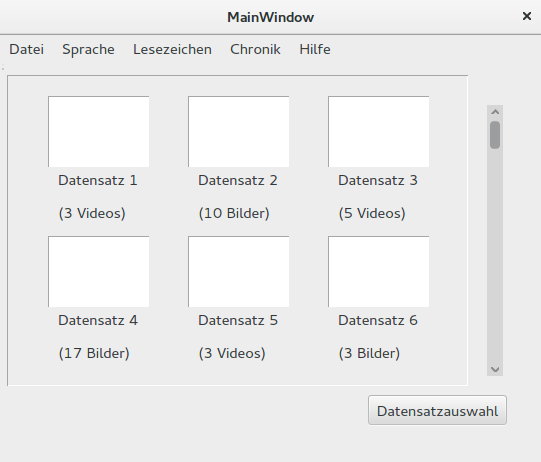
\includegraphics[width=1\linewidth]{img/Bibliothek}
Das erste Fenster beinhaltet die Bibliothek und außerdem ein Menü. In der Menüleiste kann im Punkt Datei ein neuer Datensatz ausgewählt oder das Programm beendet werden.  Unter Sprache kann die aktuelle Sprache ausgewählt werden. Unter Lesezeichen können Suchergebnisse geöffnet werden, die als Lesezeichen gespeichert wurden. In der Chronik kann ein Suchergebnis der letzten 5 Suchen geöffnet werden. Über den Menüpunkt Hilfe kann eine Anleitung oder ein About-Fenster geöffnet werden.
In der Bibliothek befinden sich die Datensätze aus dem Standardordner und zuletzt verwendete. Daraus kann ein Datensatz ausgewählt werden, in dem sich das Bild/Video befindet, nach dem gesucht werden soll. Mithilfe des Buttons \enquote{neuer Datensatz} kann auch ein anderer Ordner als Datensatz gewählt werden.

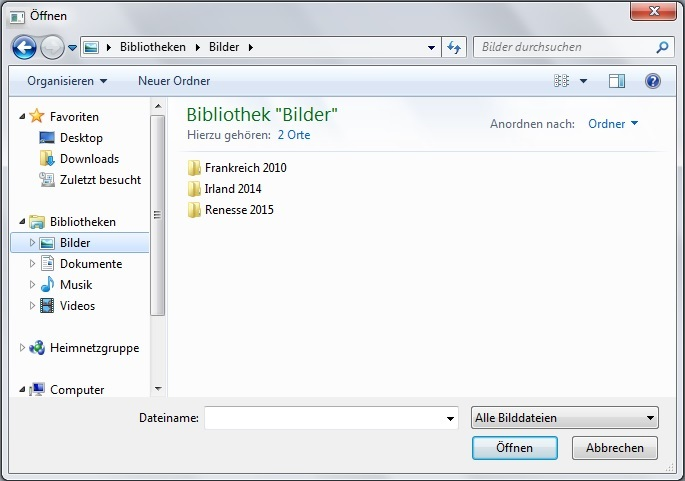
\includegraphics[width=1\linewidth]{img/FileChooser}
Hier kann der Benutzer einen Bild- oder Videodatensatz auswählen.

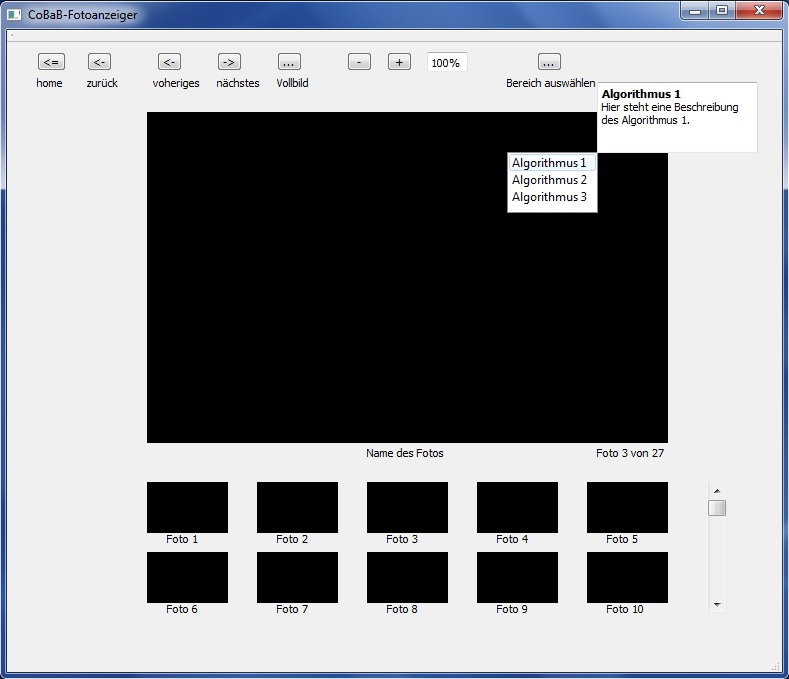
\includegraphics[width=1\linewidth]{img/Fotoanzeiger}
Über den \enquote{Home} Button oben links kommt der Benutzer zurück zur Bibliothek. Beim Klicken des \enquote{zurück} Buttons kann ein Schritt rückgängig gemacht werden, man kommt also zum vorherigen Fenster. Diese Buttons werden in den nächsten Fenstern immer an der gleichen Stelle sein.

Nach der Auswahl eines Datensatzes öffnet sich ein Bild-/Videoanzeiger, je nach dem, ob ein Bild- oder Videodatensatz gewählt wurde. Über die Buttons \enquote{vorheriges} und \enquote{nächstes} kann der Benutzer durch die Bilder/Videos browsen und ein geeignetes auswählen. Über den Button Vollbild kann das Bild/Video im Vollbildmodus angezeigt werden.
Bei einem Rechtsklick auf das Bild werden die Algorithmen aufgelistet, die für diese Suche zur Verfügung stehen. Fährt man mit der Maus über einen solchen Algorithmus, dann erscheint eine Beschreibung zu diesem.
In den Bildern werden außerdem, falls vorhanden, Annotationen angezeigt. Davon kann eine (mit Klick darauf) ausgewählt werden. Optional kann auch ein eigenes Rechteck gezogen werden. Mit Rechtsklick auf eine Annotation erscheint eine Auswahl aller Suchalgorithmen, die für diese Annotation in Frage kommen. Der Benutzer kann durch Klicken auf einen Algorithmusnamen mit dem Programm fortfahren.

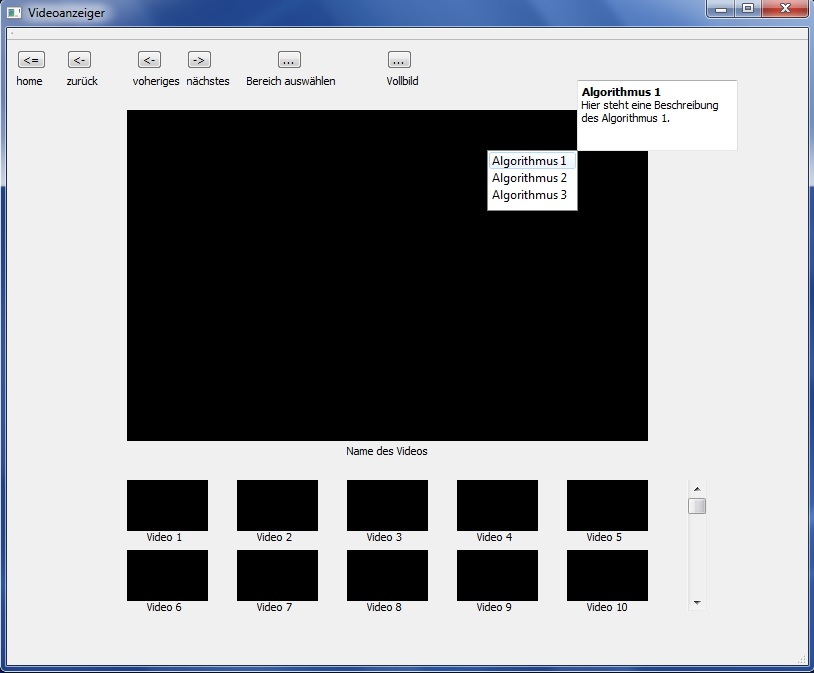
\includegraphics[width=1\linewidth]{img/Videoanzeiger}
Der Videoanzeiger bietet alle Funktionen des oben beschriebenen Fotoanzeigers. Zusätzlich können auch Videos abgespielt werden. Dabei wird im Player, ähnlich zu YouTube, Play, Pause, ein Fortschrittsbalken und die vergangene Zeit angezeigt. 

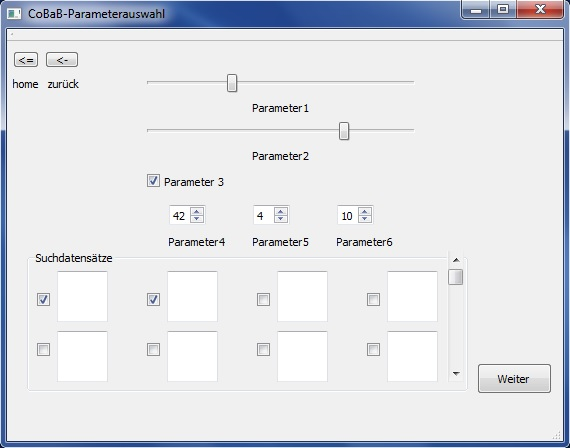
\includegraphics[width=1\linewidth]{img/Parameterauswahl}
Nach der Auswahl eines Suchverfahrens, kann man Parameter für den Suchalgorithmus festlegen. Außerdem können weitere Datensätze ausgewählt werden, in denen gesucht werden soll.

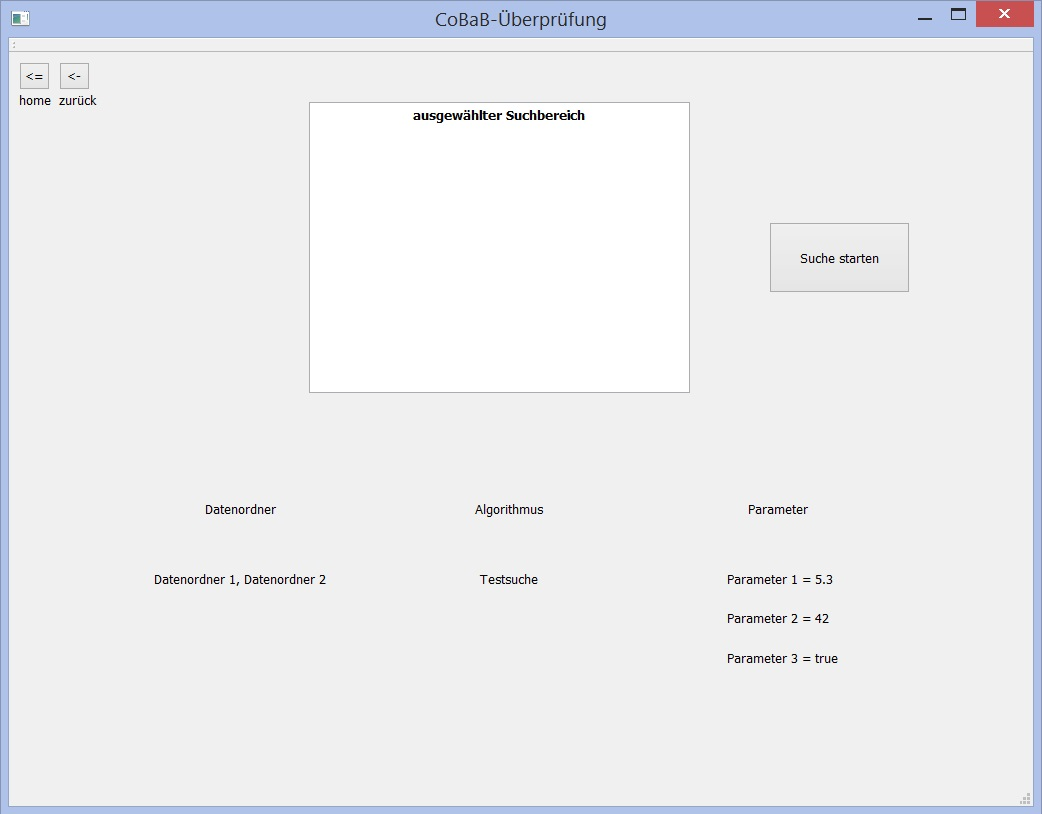
\includegraphics[width=1\linewidth]{img/Ueberpruefung}
Im Überprüfungsfenster wird noch einmal die aktuelle Auswahl angezeigt: der gewählte Bild-/Videoausschnitt, die Datensätze, in denen gesucht wird, der Suchalgorithmus und die Parameter. Wenn der Benutzer an diesen Werten nichts mehr ändern will, kann er nun über den Button \enquote{Suche starten} das Suchverfahren mit der gezeigten Auswahl starten.

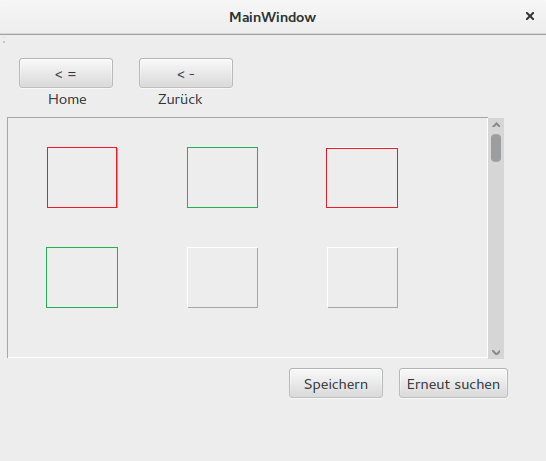
\includegraphics[width=1\linewidth]{img/Suchergebnisse}
Während der Suche wird eine Fortschrittsanimation in dem Fenster angezeigt, in dem dann die Suchergebnisse zu sehen sein werden. Wenn alle Ergebnisse angezeigt werden, kann das Suchergebnis über den Button als Lesezeichen gespeichert werden.\newline 
Der Benutzer kann durch einen Klick auf ein Bild dieses als positiv (grüner Kasten) bewerten. Durch einen weiteren Klick wird es negativ (roter Kasten) und durch noch einen Klick wieder neutral (kein Kasten) bewertet. Durch einen Klick auf den Button \enquote{Erneut suchen}, wird das Feedback an den Algorithmus übermittelt und eine neue verbesserte Suche gestartet.
\pagebreak
